% Group dynamics: classifying disagreement, then three scenarios for the room.
% Shared preamble for the write-on class slides.
%
% Every deck is designed to be projected and annotated live on a tablet:
% whatever takes time to draw is pre-drawn, and whatever the class produces is
% left blank. Compile a deck with `pdflatex main.tex` from its own directory,
% or run `uv run python build.py` from the repository root to build them all.
\documentclass[10pt]{article}

\usepackage[papersize={25.6cm,14.4cm}, margin=1.1cm, bottom=1.5cm,
            footskip=0.75cm]{geometry}
\usepackage[T1]{fontenc}
\usepackage[default]{sourcesanspro}
\usepackage{newtxsf}
\usepackage{tikz}
\usepackage{amsmath}
\usepackage{parskip}
\usepackage{fancyhdr}
\usetikzlibrary{arrows.meta, positioning, calc}

\setlength{\parindent}{0pt}

% Catppuccin Latte, the palette the course site uses in its light theme, so a
% deck on the projector looks like the pages the students read.
\definecolor{inkbg}{HTML}{EFF1F5}      % base
\definecolor{inksurface}{HTML}{E6E9EF} % mantle
\definecolor{inkfaint}{HTML}{CCD0DA}   % surface2, for rules and empty boxes
\definecolor{inktext}{HTML}{4C4F69}    % text
\definecolor{inkgrey}{HTML}{8C8FA1}    % overlay1, for anything secondary
\definecolor{inkblue}{HTML}{7287FD}    % lavender, the primary accent
\definecolor{inkteal}{HTML}{179299}    % teal
\definecolor{inkred}{HTML}{FE640B}     % peach, for whatever wants attention
\definecolor{inkmauve}{HTML}{8839EF}   % mauve

\pagecolor{inkbg}
\color{inktext}

% A box to write a short answer into. White against the tinted page, so it
% reads as somewhere to write rather than as part of the printed material.
\newcommand{\blank}[1][1.6]{%
  \tikz[baseline=(current bounding box.base)]{%
    \draw[inkfaint, line width=0.7pt, rounded corners=2pt, fill=white]
      (0,-0.18) rectangle (#1,0.62);}}

% A ruled area to work in. Faint dots keep handwriting level on a tablet.
\newcommand{\workspace}[2]{%
  \begin{tikzpicture}
    \draw[inkfaint, line width=0.7pt, rounded corners=3pt, fill=white]
      (0,0) rectangle (#1,#2);
    \foreach \gx in {0.5,1.0,...,#1}{%
      \foreach \gy in {0.5,1.0,...,#2}{%
        \fill[inkfaint] (\gx,\gy) circle (0.5pt);}}
  \end{tikzpicture}}

% A panel for material that is printed rather than written on.
\newcommand{\panel}[2]{%
  \begin{tikzpicture}
    \draw[inkfaint, line width=0.7pt, rounded corners=3pt, fill=inksurface]
      (0,0) rectangle (#1,#2);
  \end{tikzpicture}}

% A labelled card of printed material. #2 and #3 are widths in cm; the text
% column is the card less its padding, computed rather than guessed.
\newcommand{\cardbox}[4]{%
  \begin{tikzpicture}
    \node[draw=#1, line width=1pt, rounded corners=4pt, fill=white,
          minimum width=#2cm, minimum height=#3cm,
          text width=\dimexpr#2cm-0.9cm\relax,
          align=left, inner sep=0.45cm, text=inktext] {#4};
  \end{tikzpicture}}

% A card whose body is left blank for the class to fill in.
\newcommand{\cardblank}[4]{%
  \begin{tikzpicture}
    \node[draw=#1, line width=1pt, rounded corners=4pt, fill=white,
          minimum width=#2cm, minimum height=#3cm,
          text width=\dimexpr#2cm-0.9cm\relax,
          align=left, inner sep=0.45cm, text=inktext, anchor=north west]
      at (0,0) {#4};
  \end{tikzpicture}}

% Running header: the deck name on the left, the page's own step on the right.
% Each deck sets its name once with \deckname.
\newcommand{\deck}{}
\newcommand{\deckname}[1]{\renewcommand{\deck}{#1}}
\newcommand{\slidehead}[1]{%
  {\small\color{inkgrey}%
   \tikz[baseline=-0.5ex]{\fill[inkblue, rounded corners=1pt]
     (0,0) rectangle (0.22,0.22);}\;\deck
   \hfill \color{inkblue}\bfseries #1}\par
  {\color{inkblue}\rule{\linewidth}{1pt}}\par\vspace{0.35em}}

\pagestyle{fancy}
\fancyhf{}
\renewcommand{\headrulewidth}{0pt}
\fancyfoot[R]{\small\color{inkgrey}\thepage}

% Deck title pages, which carry no header and no page number.
\newcommand{\titleslide}[3]{%
  \thispagestyle{empty}%
  \begin{center}
    \vspace*{\fill}
    {\Huge\bfseries\color{inkblue} #1}\\[0.7em]
    {\LARGE\color{inkgrey} #2}\\[2.4em]
    #3
    \vspace*{\fill}
  \end{center}}

% One step of the plan on a title page.
\newcommand{\stepbox}[3]{%
  \node[draw=inkblue, line width=0.9pt, rounded corners=4pt, fill=white,
        minimum width=6cm, minimum height=1.7cm, align=center,
        text=inktext] (#1) at (#2,0) {#3};}

% Prompt to the room: a question the class answers, not something I read out.
\newcommand{\ask}[1]{%
  {\large\color{inkblue}\bfseries #1}\par\vspace{0.5em}}


\deckname{Group dynamics}

\begin{document}

\titleslide{Group dynamics}{Disagreement is normal. Handling it is a skill.}{%
    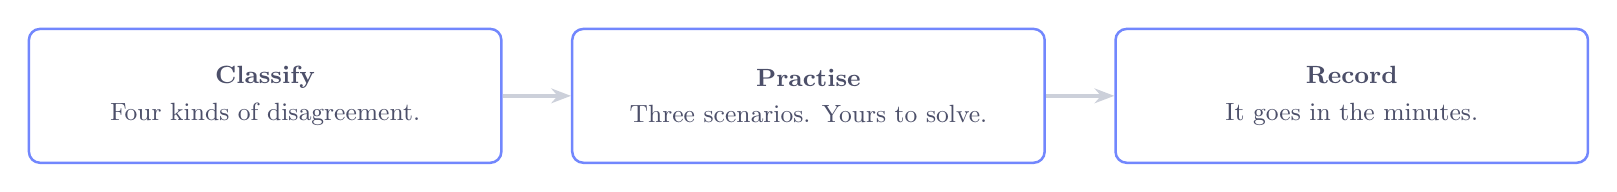
\begin{tikzpicture}[font=\small]
      \stepbox{s0}{0.0}{\textbf{Classify}\\[0.25em] Four kinds of disagreement.}
      \stepbox{s1}{6.9}{\textbf{Practise}\\[0.25em] Three scenarios. Yours to solve.}
      \stepbox{s2}{13.8}{\textbf{Record}\\[0.25em] It goes in the minutes.}
      \draw[-{Stealth[length=2.5mm]}, inkfaint, line width=1.2pt] (s0) -- (s1);
      \draw[-{Stealth[length=2.5mm]}, inkfaint, line width=1.2pt] (s1) -- (s2);
    \end{tikzpicture}}

\newpage
\slidehead{Start here}

\vspace{1.5cm}

\begin{center}
{\Huge\bfseries\color{inkblue} Disagreement is normal.}

\vspace{1.8cm}

{\LARGE A group that never disagrees is either dominated\\
by one person, or not engaging with the work.}
\end{center}

\newpage
\slidehead{Four kinds, and what each one needs}

\vspace{0.6cm}

\begin{center}
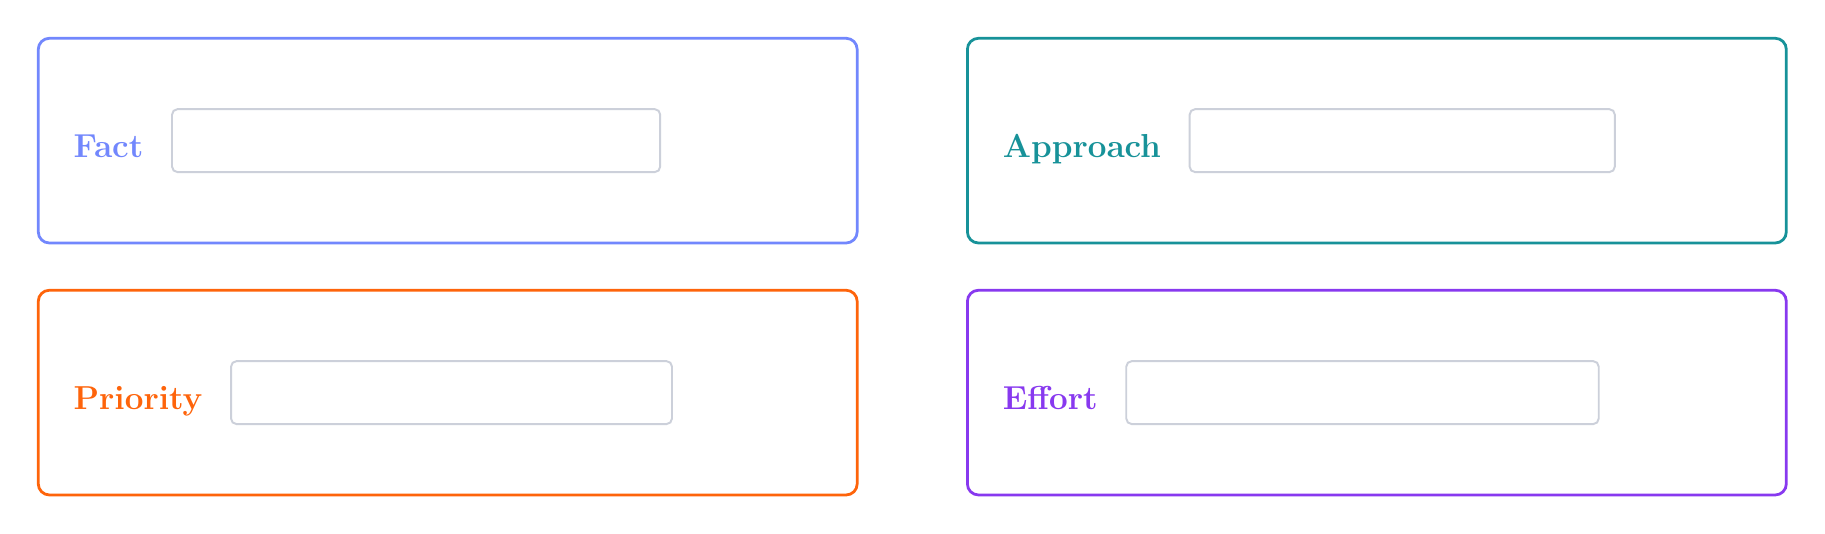
\begin{tikzpicture}
  \node at (0,0) {\cardbox{inkblue}{10.4}{2.6}{%
    {\large\bfseries\color{inkblue} Fact}\quad\blank[6.2]}};
  \node at (11.8,0) {\cardbox{inkteal}{10.4}{2.6}{%
    {\large\bfseries\color{inkteal} Approach}\quad\blank[5.4]}};
  \node at (0,-3.2) {\cardbox{inkred}{10.4}{2.6}{%
    {\large\bfseries\color{inkred} Priority}\quad\blank[5.6]}};
  \node at (11.8,-3.2) {\cardbox{inkmauve}{10.4}{2.6}{%
    {\large\bfseries\color{inkmauve} Effort}\quad\blank[6.0]}};
\end{tikzpicture}
\end{center}

\vspace{0.4cm}

\ask{How would you settle each one?}

\newpage
\slidehead{The framework}

\vspace{1.3cm}

\begin{center}
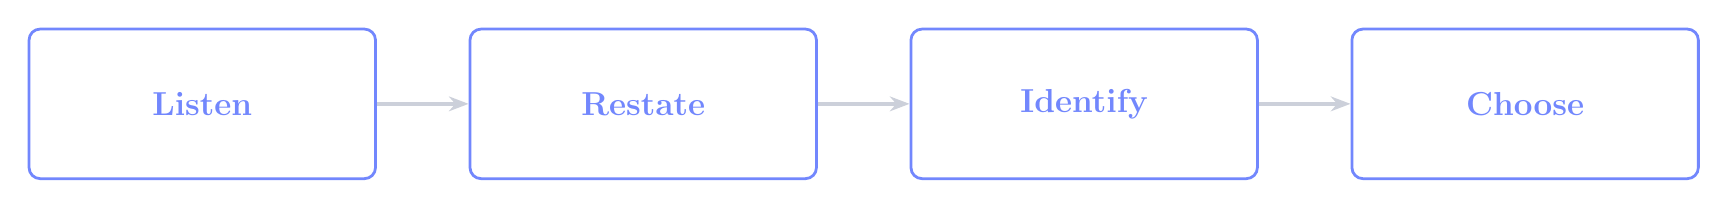
\begin{tikzpicture}
  \foreach \w/\x in {Listen/0, Restate/5.6, Identify/11.2, Choose/16.8}{%
    \node[draw=inkblue, line width=1pt, rounded corners=4pt, fill=white,
          minimum width=4.4cm, minimum height=1.9cm, font=\large\bfseries,
          text=inkblue] (\w) at (\x,0) {\w};}
  \foreach \a/\b in {Listen/Restate, Restate/Identify, Identify/Choose}{%
    \draw[-{Stealth[length=2.5mm]}, inkfaint, line width=1.3pt] (\a) -- (\b);}
\end{tikzpicture}
\end{center}

\vspace{1.5cm}

\begin{center}
{\LARGE \textbf{Restate} is the one everybody skips.}
\end{center}

\newpage
\slidehead{Scenario 1}

\vspace{0.3cm}

\begin{minipage}[t]{0.44\linewidth}
\vspace{0pt}
{\large
B wants the tests written before the functions.\\[0.6em]
C wants the library first, then the tests.\\[0.6em]
\textcolor{inkred}{Neither will move. Fifteen minutes gone.}}
\end{minipage}
\hfill
\begin{minipage}[t]{0.52\linewidth}
\vspace{0pt}
\ask{Which kind? What happens next?}

\workspace{11.8}{5.6}
\end{minipage}

\vspace{0.3cm}

{\large Into the minutes: \blank[12]}

\newpage
\slidehead{Scenario 2}

\vspace{0.3cm}

\begin{minipage}[t]{0.44\linewidth}
\vspace{0pt}
{\large
A: ``it runs without an error, so it is correct''.\\[0.6em]
D: ``it is wrong''.\\[0.6em]
\textcolor{inkred}{Ten minutes. Both getting irritated.}}
\end{minipage}
\hfill
\begin{minipage}[t]{0.52\linewidth}
\vspace{0pt}
\ask{Which kind? What do they do right now?}

\workspace{11.8}{5.6}
\end{minipage}

\vspace{0.3cm}

{\large How long should this have taken? \blank[6]}

\newpage
\slidehead{Scenario 3}

\vspace{0.3cm}

\begin{minipage}[t]{0.44\linewidth}
\vspace{0pt}
{\large
D's function is still not written.\\[0.6em]
Second week running.\\[0.6em]
\textcolor{inkred}{Two members are messaging each other
privately about it.}}
\end{minipage}
\hfill
\begin{minipage}[t]{0.52\linewidth}
\vspace{0pt}
\ask{Which kind? What is wrong with the messages?}

\workspace{11.8}{5.6}
\end{minipage}

\newpage
\slidehead{Effort: say it like this}

\vspace{0.7cm}

\begin{center}
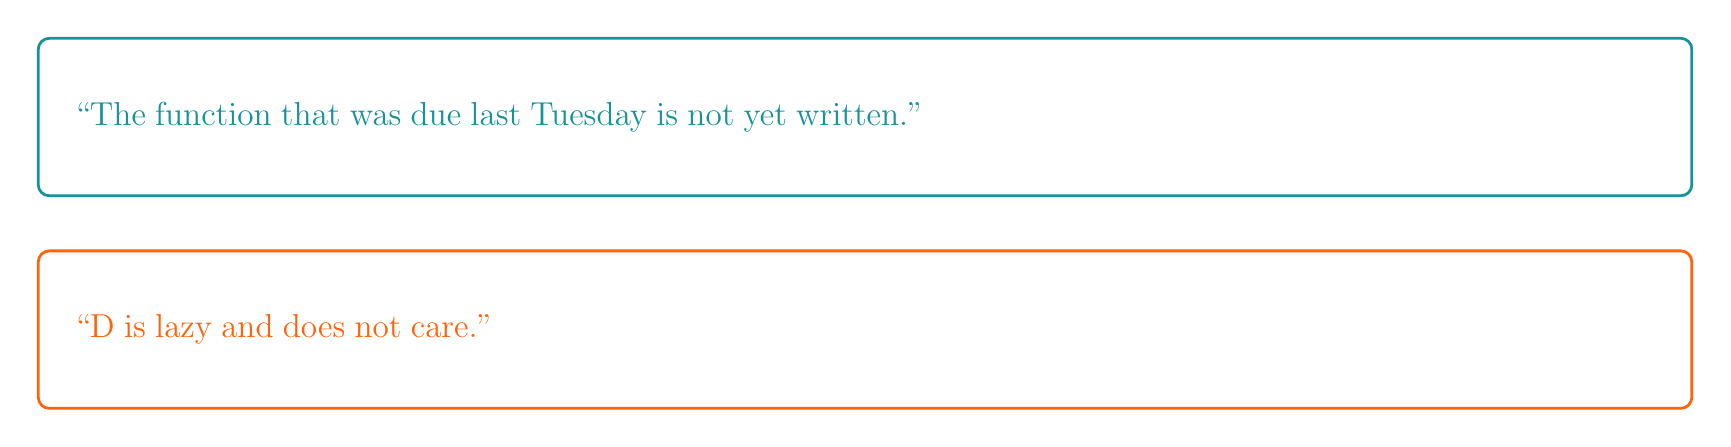
\begin{tikzpicture}
  \node at (0,0) {\cardbox{inkteal}{21}{2.0}{%
    {\large\color{inkteal} ``The function that was due last Tuesday is not
     yet written.''}}};
  \node at (0,-2.7) {\cardbox{inkred}{21}{2.0}{%
    {\large\color{inkred} ``D is lazy and does not care.''}}};
\end{tikzpicture}
\end{center}

\vspace{0.7cm}

\begin{center}
{\LARGE In a meeting. Not outside one.}
\end{center}

\newpage
\slidehead{The chair, every week}

\vspace{1.2cm}

{\LARGE
\textbf{\color{inkblue}1.}\quad \textbf{Round-robin} the discussion.
Anyone may pass.

\vspace{1.2em}

\textbf{\color{inkblue}2.}\quad \textbf{Check each decision} one member at
a time. A nod is not enough.}

\vspace{1.6cm}

\begin{center}
{\LARGE Artificial the first time. Ordinary by week three.}
\end{center}

\newpage
\slidehead{When it stalls}

\vspace{1.0cm}

{\LARGE
Take a \textbf{break}. \qquad
\textbf{Try both} for a week.

\vspace{1.2em}

\textbf{Defer} to the chair. \qquad
\textbf{Write it down}, one sentence each.}

\vspace{1.6cm}

\begin{center}
{\LARGE It goes in the minutes either way: resolved, or still open.}
\end{center}

\newpage
\slidehead{Before you leave}

\vspace{0.8cm}

\begin{center}
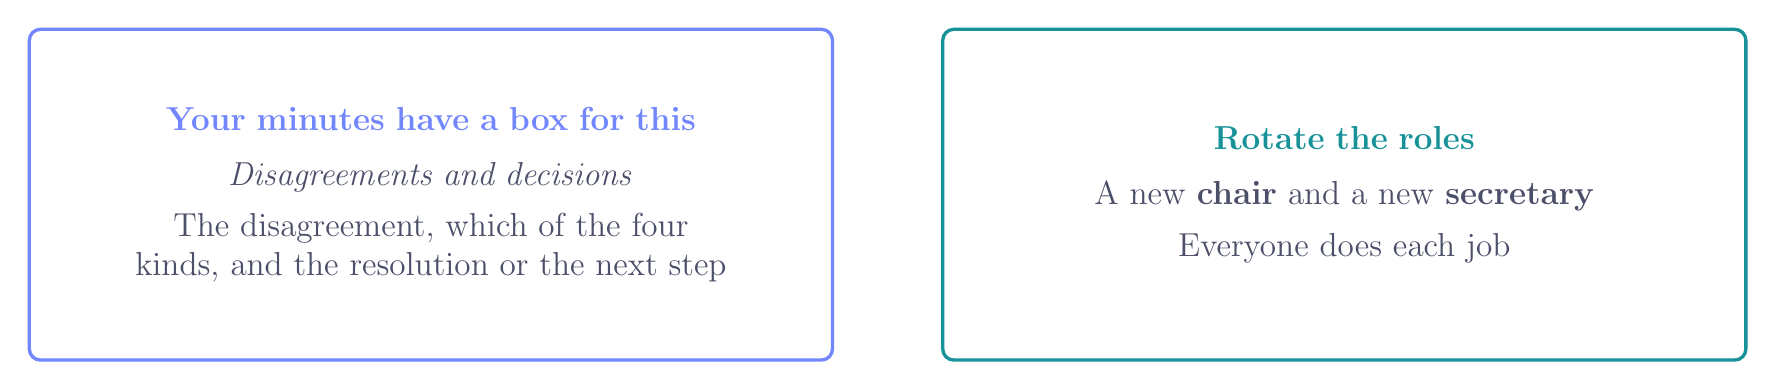
\begin{tikzpicture}
  \node[draw=inkblue, line width=1.2pt, rounded corners=4pt, fill=white,
        minimum width=10.2cm, minimum height=4.2cm, text width=9.2cm,
        align=center, inner sep=0.4cm, text=inktext, font=\large] at (0,0) {%
    \textbf{\color{inkblue} Your minutes have a box for this}\\[0.5em]
    \emph{Disagreements and decisions}\\[0.4em]
    The disagreement, which of the four kinds, and the resolution or the
    next step};
  \node[draw=inkteal, line width=1.2pt, rounded corners=4pt, fill=white,
        minimum width=10.2cm, minimum height=4.2cm, text width=9.2cm,
        align=center, inner sep=0.4cm, text=inktext, font=\large]
    at (11.6,0) {%
    \textbf{\color{inkteal} Rotate the roles}\\[0.5em]
    A new \textbf{chair} and a new \textbf{secretary}\\[0.4em]
    Everyone does each job};
\end{tikzpicture}
\end{center}

\vspace{0.9cm}

\begin{center}

\begin{tikzpicture}
  \node[draw=inkred, line width=1.4pt, rounded corners=4pt, fill=white,
        minimum width=21.8cm, minimum height=2.2cm, text width=20.6cm,
        align=center, inner sep=0.35cm, text=inktext, font=\large] {%
    \textbf{\color{inkred} Meet this week. Bring the Week 5 minutes to
    the next session.}\quad The second of the five that \(I\) is
    counted from.};
\end{tikzpicture}
\end{center}

\end{document}
